\documentclass[12pt]{article}
\usepackage[letterpaper,margin=0.7in,headheight=15pt,headsep=16pt,footskip=25pt]{geometry}
\usepackage{tikz,array,fancyhdr,lmodern}
\renewcommand{\familydefault}{\sfdefault}
\pagestyle{fancy}\fancyhf{}\renewcommand{\headrulewidth}{0.35pt}
\fancyhead[L]{\small Week 28 / Flat folds encore / Grades K--5}
\fancyfoot[L]{\scriptsize Bellingham Math Circle / Week 28 / W28-BON-v1}\fancyfoot[R]{\scriptsize\thepage}
\setlength{\parindent}{0pt}\setlength{\parskip}{9pt}
\newcommand{\problem}[2]{\par\textbf{Problem #1:} #2\par}
\newcommand{\lines}[1]{\foreach \y in {1,...,#1}{\par\vspace{20pt}\hrule height 0.3pt\relax}}
\newcommand{\alignsquare}[3]{\begin{tikzpicture}[x=0.85cm,y=0.85cm]\draw (0,0) rectangle (6,6);\foreach \l/\x/\y in {#2}{\fill (\x,\y) circle(0.075);\node[above right,inner sep=2pt] at (\x,\y){\l};}#3\node[anchor=north west] at (0,-0.2){#1};\end{tikzpicture}}
\newcommand{\pattern}[2]{\begin{tikzpicture}[x=0.78cm,y=0.78cm]\draw (-3,-3) rectangle (3,3);\draw[dashed,gray] (-3,0)--(3,0) (0,-3)--(0,3);\foreach \x/\y in {#2}\draw[fill=white,thick] (\x,\y) circle (0.09);\node at (0,-3.6){#1};\end{tikzpicture}}
\newcommand{\foldrecord}{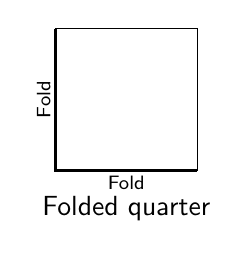
\begin{tikzpicture}[x=0.6cm,y=0.6cm]\draw (0,0) rectangle (3,3);\draw[thick] (0,3)--(0,0)--(3,0);\node[rotate=90,font=\scriptsize] at (-0.25,1.5){Fold};\node[font=\scriptsize] at (1.5,-0.25){Fold};\node at (1.5,-0.8){Folded quarter};\end{tikzpicture}}
\begin{document}
\problem{1}{Trace each picture onto a separate square of thin paper. Make one straight fold that brings P onto Q and R onto S at the same time. Where T is shown, T must stay in its original place. Draw a crease that works, or explain why none can.}
\vspace{8pt}
\alignsquare{1}{P/1/1,Q/5/1,R/2/4,S/4/4}{}\hfill\alignsquare{2}{P/1/1,Q/5/1,R/1/4,S/4/4}{}
\par\vspace{18pt}
\alignsquare{3}{P/1/1,Q/5/1,R/2/4,S/4/4,T/3/5}{}\hfill\alignsquare{4}{P/1/1,Q/5/1,R/2/4,S/4/4,T/2/5}{}
\vspace{10pt}
\lines{4}
\newpage
A strip's equal square panels stay connected. Fold only at the joins. Read a stack from top to bottom.
\begin{center}
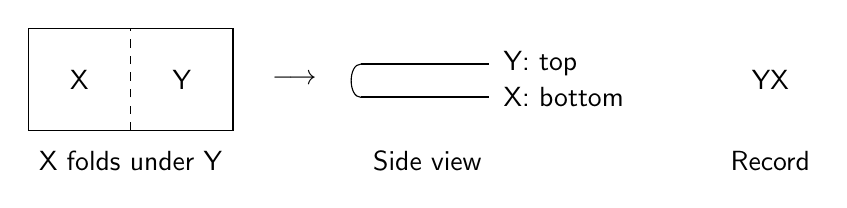
\begin{tikzpicture}[x=0.65cm,y=0.65cm]
\draw (0,0) rectangle (4,2);\draw[dashed] (2,0)--(2,2);\node at (1,1){X};\node at (3,1){Y};\node at (2,-0.6){X folds under Y};
\node at (5.2,1){$\longrightarrow$};
\draw[thick] (6.5,1.3)--(9,1.3);\draw[thick] (6.5,0.65)--(9,0.65);\draw (6.5,1.3) to[out=180,in=180] (6.5,0.65);
\node[right] at (9.1,1.3){Y: top};\node[right] at (9.1,0.65){X: bottom};\node at (7.8,-0.6){Side view};\node at (14.5,1){YX};\node at (14.5,-0.6){Record};
\end{tikzpicture}
\end{center}
Keep the original front marked. ``Toward the front'' and ``toward the back'' refer to that original front at each join.\par Read this three-panel stack with B's original front facing up.\par
\problem{2}{Fold a three-panel strip completely flat into a one-square stack. Find every top-to-bottom order of A, B, C. Can the same directions at both joins give different layer orders?}
\begin{center}
\begin{tikzpicture}[x=1.1cm,y=1.1cm]\draw (0,0) rectangle (6,2);\draw[dashed] (2,0)--(2,2) (4,0)--(4,2);\node at (1,1){A};\node at (3,1){B};\node at (5,1){C};\end{tikzpicture}
\end{center}
\begin{tabular}{|p{2.7in}|p{2.7in}|}\hline Layer order&Directions at the two joins\\\hline\rule{0pt}{39pt}&\\\hline\rule{0pt}{39pt}&\\\hline\rule{0pt}{39pt}&\\\hline\rule{0pt}{39pt}&\\\hline\rule{0pt}{39pt}&\\\hline\rule{0pt}{39pt}&\\\hline\end{tabular}
\lines{2}
\newpage
\problem{3}{Arrange A, B, C, D as four thin layers in a flat stack. In a side view, joins AB and CD bend around the same end; join BC bends around the other end. Joining bends at the same end cannot cross. Find every layer order that obeys this rule.}
\begin{center}
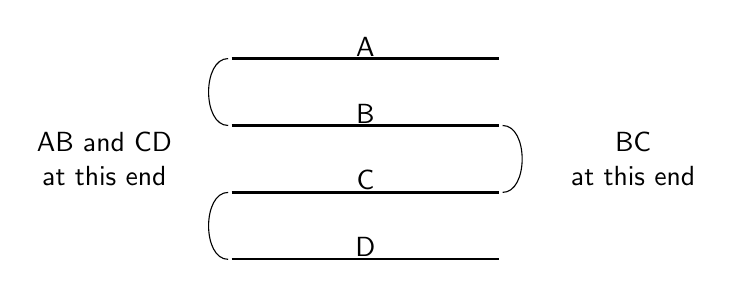
\begin{tikzpicture}[x=0.85cm,y=0.85cm]
\foreach \l/\y in {A/3,B/2,C/1,D/0}{\draw[thick] (0,\y)--(4,\y);\node at (2,\y+0.18){\l};}
\draw (-0.05,3) to[out=180,in=180] (-0.05,2);\draw (-0.05,1) to[out=180,in=180] (-0.05,0);\draw (4.05,2) to[out=0,in=0] (4.05,1);
\node[align=center] at (-1.9,1.5){AB and CD\\at this end};\node[align=center] at (6,1.5){BC\\at this end};
\end{tikzpicture}
\end{center}
This is an ideal thin-paper side view. A noncrossing drawing does not supply a folding motion with real paper.\par
\begin{tabular}{|p{1.18in}|p{1.18in}|p{1.18in}|p{1.18in}|}\hline\rule{0pt}{42pt}&&&\\\hline\rule{0pt}{42pt}&&&\\\hline\rule{0pt}{42pt}&&&\\\hline\rule{0pt}{42pt}&&&\\\hline\rule{0pt}{42pt}&&&\\\hline\rule{0pt}{42pt}&&&\\\hline\end{tabular}
\lines{3}
\newpage
A punch goes through every layer. Unfold the paper to see its pattern.
\begin{center}
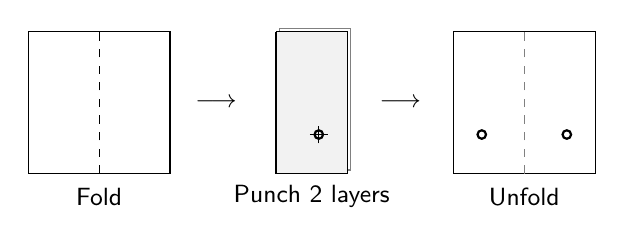
\begin{tikzpicture}[x=0.45cm,y=0.45cm,font=\small]
\draw (0,0) rectangle (4,4);\draw[dashed] (2,0)--(2,4);\node at (2,-0.65){Fold};
\node at (5.3,2){$\longrightarrow$};
\draw[gray] (7.1,0.1) rectangle (9.1,4.1);\draw[fill=gray!10] (7,0) rectangle (9,4);\draw[thick] (7,0)--(7,4);
\draw[thick] (8.2,1.1) circle (0.12);\draw (7.95,1.1)--(8.45,1.1) (8.2,0.85)--(8.2,1.35);\node at (8,-0.65){Punch 2 layers};
\node at (10.5,2){$\longrightarrow$};
\draw (12,0) rectangle (16,4);\draw[dashed,gray] (14,0)--(14,4);\draw[thick] (12.8,1.1) circle (0.12);\draw[thick] (15.2,1.1) circle (0.12);\node at (14,-0.65){Unfold};
\end{tikzpicture}
\end{center}
\problem{4}{Fold a square on its vertical and horizontal midlines into a quarter-square. Keep the top-right quarter underneath. With an adult, make one punch through every layer, away from folds and edges. Which patterns below can come from that one punch? Mark the punch position on the folded quarter for each possible pattern.}
\begin{center}
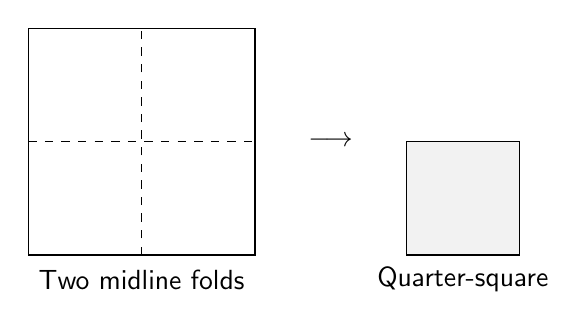
\begin{tikzpicture}[x=0.48cm,y=0.48cm]
\draw (0,0) rectangle (6,6);\draw[dashed] (3,0)--(3,6) (0,3)--(6,3);\node at (3,-0.65){Two midline folds};\node at (8,3){$\longrightarrow$};
\draw[fill=gray!10] (10,0) rectangle (13,3);\node at (11.5,-0.65){Quarter-square};
\end{tikzpicture}
\end{center}
\pattern{1}{1.7/.9,1.7/-.9,-1.7/.9,-1.7/-.9}\hfill\pattern{2}{1.2/1.2,1.2/-1.2,-1.2/1.2,-1.2/-1.2}\hfill\pattern{3}{1.7/.9,1.7/-.9,-1.7/.9,-1.2/-.9}
\par\vspace{18pt}
\foldrecord\hfill\foldrecord\hfill\foldrecord
\vspace{16pt}
\lines{4}
\newpage
\problem{5}{Fold the quarter-square from Problem 4 along its diagonal, making a triangle. Punch once through every layer, away from every fold and edge. Which patterns below can come from one punch? Mark a punch position for each possible pattern, or explain why it cannot work.}
\begin{center}
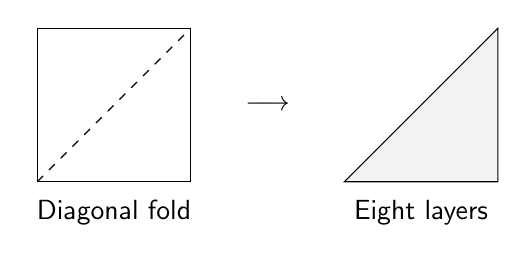
\begin{tikzpicture}[x=0.65cm,y=0.65cm]\draw (0,0) rectangle (3,3);\draw[dashed] (0,0)--(3,3);\node at (1.5,-0.6){Diagonal fold};\node at (4.5,1.5){$\longrightarrow$};\draw[fill=gray!10] (6,0)--(9,0)--(9,3)--cycle;\node at (7.5,-0.6){Eight layers};\end{tikzpicture}
\end{center}
\pattern{1}{1.7/.9,1.7/-.9,-1.7/.9,-1.7/-.9,.9/1.7,.9/-1.7,-.9/1.7,-.9/-1.7}\hfill\pattern{2}{1.8/.7,1.8/-.7,-1.8/.7,-1.8/-.7,.7/1.8,.7/-1.8,-.7/1.8,-.7/-1.8}\hfill\pattern{3}{1.7/.8,1.7/-.8,-1.7/.8,-1.7/-.8,.7/1.4,.7/-1.4,-.7/1.4,-.7/-1.4}
\par\vspace{18pt}
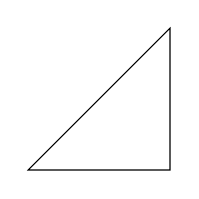
\begin{tikzpicture}[x=0.6cm,y=0.6cm]\draw (0,0)--(3,0)--(3,3)--cycle;\end{tikzpicture}\hfill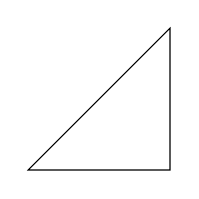
\begin{tikzpicture}[x=0.6cm,y=0.6cm]\draw (0,0)--(3,0)--(3,3)--cycle;\end{tikzpicture}\hfill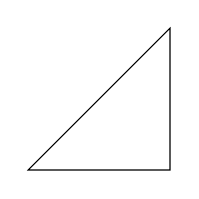
\begin{tikzpicture}[x=0.6cm,y=0.6cm]\draw (0,0)--(3,0)--(3,3)--cycle;\end{tikzpicture}
\vspace{16pt}
\lines{7}
\end{document}
